\documentclass{elsarticle}
\usepackage{graphicx}
%\usepackage{multicol}
%\usepackage{footmisc}
\usepackage{amstext}
\usepackage{amsmath}
\usepackage{amssymb}
\usepackage[english]{babel}
%\usepackage[official,right]{eurosym}
\selectlanguage{english}
% Ampersand -----------------------------------------------------------

\def\id#1{\text{\em #1\/}}
\newcommand{\code}[1]{\text{\tt\small #1}}
\newcommand{\stmtText}[1]{``{\small\tt #1}''}
\newcommand{\dom}[1]{\id{dom}(#1)}
\newcommand{\cod}[1]{\id{cod}(#1)}
\renewcommand{\int}[2]{\id{inter}(#1,#2)}
\newcommand{\pop}[1]{\id{pop}(#1)}
\newcommand{\src}[1]{\id{src}(#1)}
\newcommand{\trg}[1]{\id{trg}(#1)}
\newcommand{\powerset}[1]{\cal{P}\{#1\}}
\newcommand{\theCode}{\url{http://cs.ru.nl/~B.Joosten/ampTypes/}}
\newcommand{\la}{\langle}
\newcommand{\ra}{\rangle}
\newcommand{\full}{V}
\newcommand{\declare}[3]{\id{#1}_{\pair{\id{\small #2}}{\id{\small #3}}}}
\newcommand{\fullt}[2]{V_{\pair{#1}{#2}}}
\newcommand{\iden}[1]{I}
\newcommand{\ident}[1]{I_{\id{\small #1}}}
\newcommand{\expr}[3]{(#1)_{#2\times #3}}
\newcommand{\pair}[2]{\la{#1},{#2}\ra}
\newcommand{\atom}[1]{{\tt\small #1}}
\newcommand{\atoms}{\mathcal{A}}
\newcommand{\concepts}{\mathcal{C}}
\newcommand{\decls}{\mathcal{D}}  %% names of relations
\newcommand{\rels}{\mathcal{R}}   %% all relations
\newcommand{\relations}{\mathcal{M}} % representing terms. M is a subset of R.
\newcommand{\terms}{\mathcal{T}}
\newcommand{\vertices}{N}
\newcommand{\rules}{\mathcal{H}}
\newcommand{\tf}[1]{\mathfrak{T}(#1)}
\newcommand{\ptf}[1]{\mathfrak{T}'(#1)}
\newcommand{\ti}[1]{\mathfrak{I}(#1)}
\newcommand{\tic}[1]{I_{\cal C}(#1)}
\newcommand{\relAdd}{\dagger}
\newcommand{\flip}[1]{{#1}^\smallsmile} %formerly:  {#1}^\backsim
\newcommand{\kleeneplus}[1]{{#1}^+}
\newcommand{\kleenestar}[1]{{#1}^*}
\newcommand{\cmpl}[1]{\overline{#1}}
\newcommand{\rel}{\times}
\newcommand{\compose}{;}
\newcommand{\subs}{\subseteq}%{\models}
\newcommand{\fun}{\rightarrow}
\newcommand{\isa}{\preceq}
%\newcommand{\isaClos}{\sqsubseteq}
\newcommand{\typetest}{?}
\newcommand{\meet}{\sqcap}
\newcommand{\join}{\sqcup}
\newcommand{\Meet}{\bigsqcap}
\newcommand{\Moin}{\bigsqcup} % because LaTeX has already defined command \Join.
\newcommand{\order}{\ominus}
\newcommand{\anything}{\top}
\newcommand{\nothing}{\bot}
\newcommand{\rewriteto}{\rightarrow}
\newcommand{\calc}{\implies}
\newcommand{\alland}{\bigwedge}
\newcommand{\mph}[3]{#1_{#2\times #3}}
\newcommand{\mphu}[1]{#1_{\univ\times\univ}}

%-----------------------------------------
\newcommand{\kse}{\hspace*{1.7em}}
\newcommand{\ksf}{\hspace*{1em}}
\newcommand{\ksg}{\hspace*{1em}}
\newenvironment{derivation}{\begin{tabbing}\kse \= \ksf \= \ksg \= \kill}{\end{tabbing}}
\newtheorem{definition}{Definition}
\newcommand{\term}[1]{\>\>\(#1\)\\[1ex]}
\newcommand{\rela}[2]{\>\(#1\)\>\>\{ \ #2 \ \}\\[1ex]}
\newcommand{\weg}[1]{}

\def\define#1{\label{dfn:#1}{\em #1}\index{#1}}
\def\definem#1{\label{dfn:#1}{\em #1}\index{#1}\marge{#1}}
\newcommand{\marg}[1]{\index{#1}\marge{#1}}

\begin{document}

\title{Ampersand uses Relation Algebra as Programming Language}
\author[ou,ordina]{Stef Joosten\fnref{fn1}}
\ead{stef.joosten@ou.nl}
\address[ou]{Open Universiteit Nederland, Postbus 2960, 6401 DL Heerlen, the Netherlands}
\address[ordina]{Ordina NV,  Nieuwegein, the Netherlands}
\fntext[fn1]{ORCID 0000-0001-8308-0189}

\begin{abstract}
	Relation Algebra can be used as a programming language for building information systems.
	This paper demonstrates the principle by presenting a case study together with the theory behind programming in Relation Algebra.
	As a case study, we have developed a database-application for legal reasoning.
	We discuss a small part of it to illustrate the mechanisms of programming in Relation Algebra.
	Beside being declarative, relation algebra comes with attractive promises for developing big software.
	The compiler that was used for this case study, Ampersand, is the result of an open source project.
	Ampersand has been tried and tested in practice and is available as free open source software\footnote{\tt https://github.com/AmpersandTarski/Ampersand}.
	This article is an extended version of a conference paper presented at RAMiCS-2017 \cite{JoostenRAMiCS2017}.
\end{abstract}

\begin{keyword}
relation algebra\sep software development\sep legal reasoning\sep information systems design\sep Ampersand\sep MirrorMe\sep big software
\end{keyword}
\maketitle

\section{Introduction}
\label{sct:Introduction}
	This paper investigates how relation algebra can be used as a programming language for information systems.
	A compiler, Ampersand~\cite{Michels2011}, is used to compile concepts, relations and rules into a working database-application.
	Ampersand is a syntactically sugared version of heterogeneous relation algebra \cite{Schmidt1997}.
	We present a case study to demonstrate programming in relation algebra and its impact on the software development process.
	The case study takes the reader by the hand in the thinking process of a software developer who programs with relation algebra.

	The use of relation algebra as a programming language is not new.
	It stands in the tradition of relation algebra~\cite{Maddux06}, logic programming~\cite{Lloyd1984},
	database application programming~\cite{Codd70}, and formal specification of software.
	Ampersand uses these ideas to compile relation algebra to working software, an idea which is also found in RelView~\cite{Berghammer2005} by Berghammer (Univ. of Kiel).
 	Ampersand lets the user specify constraints only and generates an information system that respects these constraints.
	RelView also generates software but uses relational algebra as operators in an otherwise imperative programming language.
	This makes RelView stronger in specifying complex computational problems.
	Some more differences with earlier programming languages are discussed in section~\ref{sct:Comparison}.

	The author shares the belief that a provably correct implementation of requirements are essential to the software development process~\cite{Boehm1981}.
	Being fully aware of the fate of formal methods in computer science,
        Ampersand is nevertheless founded on relation algebra.
	It builds further on foundations laid by formal specification methods
	such as Z~\cite{Z} and Alloy~\cite{Alloy2006}.
	In contrast however with such methods, Ampersand is equipped with a software generator that generates an information system.
	Thus, specifying in Ampersand is developing software at the same time.

	The user may regard Ampersand as a programming language, especially suited for designing the back-end of information systems.
	The axioms of Tarski can be used to manipulate expressions in a way that preserves meaning~\cite{vdWoude2011}.
	This makes Ampersand a declarative language.

	Our case study shows an argument assistant for legal professionals, which was built as innovation project at Ordina.
	The purpose of this argument assistant is to support legal professionals in constructing a legal brief%
\footnote{A \define{brief} is a document that is meant to summarize a lawsuit for the judge and counterparty.
	It provides legal reasons for claims in a lawsuit based on regulations, precedents, and other legally acceptable sources.
	It shows how the reasoning applies to facts from the case.}.
	To the programmer, this offers the challenge to represent the problem of legal reasoning in relation algebra.
	This challenge is by no means simple, but outside the scope of this paper.
	In the Ampersand project at the Open University of the Netherlands,
	we are studying practical and didactical issues of software development in relation algebra~\cite{Michels2015}.

	The contribution of this paper is twofold.
	The case study contributes to the idea that programming can be done in relation algebra.
	The theory in section~\ref{sct:Code Fragments} contributes a theory to assist in preserving invariants.
	That theory has been consolidated in the Archive of Formal Proofs\footnote{https://www.isa-afp.org/}~\cite{Joosten-AFP17}.
	All proofs upon which this paper is based have been checked using the theorem prover Isabelle~\cite{Nipkow2002}.

	Section~\ref{sct:Ampersand} introduces Ampersand and its semantics.
	Section~\ref{sct:Conceptual analysis} introduces part of a theory of legal reasoning,
	which was developed for argument assistance.
	Section~\ref{sct:Programming in RA} discusses the programming mechanism in the application,
	and section~\ref{sct:Programming} visualizes that mechanism.
	Section~\ref{sct:Code Fragments} presents one way (of infinitely many) to derive code for arbitrary rules in relation algebra.
	Section~\ref{sct:Reflection} reflects on software development in Ampersand.
	It also provides an overview of the use of Ampersand in practice and an outlook to its further development.

\section{Ampersand}
\label{sct:Ampersand}
	In this section we explain the basics of Ampersand.
	The reader is expected to have sufficient background in relation algebra,
	in order to understand the remainder of this paper.

	The core of an Ampersand-script is a triple $\la\rules,\rels,\concepts\ra$,
	which consists of a set of rules $\rules$, relations $\rels$, and concepts $\concepts$.
	Ampersand-scripts are interpreted by the compiler as an information system.
	The rules constitute a theory in heterogeneous relation algebra.
	They constrain a body of data that resides in a database.

	The Ampersand-compiler generates a database from relations in the script.
	A database-application%
\footnote{Ampersand generates an application that consists of a relational database and interface components.
	Currently this application runs server-side on a PHP/MySQL platform and on a web-browser on the client-side.}
	assists users to keep rules satisfied throughout the lifetime of the database. It is also generated by Ampersand.

	A rule is an equality between two terms.
	Terms are built from relations.
	Ampersand interprets every relation as a finite set of pairs, which are stored in the database.
	The phase in which Ampersand takes a script, and turns it into a database, is what we will refer to as \define{compile-time}.
	The phase in which a user interacts with the database, is what we will refer to as \define{run-time}.
	At run-time, Ampersand can decide which rules are satisfied by querying the database.
	The compiler generates all software needed to keep rules satisfied at run-time.
	If a rule is not satisfied as a result of data that has changed, that change is reverted (rolled back) to
	preserve a state in which all rules are satisfied.
	Changes to the database are not specified by the software developer, but generated by the compiler.
	Rules in Ampersand are kept satisfied rather than executed directly.
	
	Atoms are values that have no internal structure, meant to represent data elements in a database.
	From a business perspective, atoms are used to represent concrete items of the world,
	such as \atom{Peter}, \atom{1}, or \atom{the king of France}.
	By convention throughout the remainder of this paper, variables $a$, $b$, and $c$ are used to represent \emph{atoms}.
	The set of all atoms is called $\atoms$.
        Each atom is an instance of a \emph{concept}.

	Concepts (from set $\concepts$) are names we use to classify atoms in a meaningful way.
	For example, you might choose to classify \atom{Peter} as a person, and \atom{074238991} as a telephone number.
        We will use variables $A$, $B$, $C$, $D$ to represent concepts.
	The term $\ident{A}$ represents the \emph{identity relation} of concept $A$.
	The expression $a \in A$ means that atom $a$ is an instance of concept $A$.
	The declaration of $A\isa B$ (pronounce: $A$ is a $B$)
	in an Ampersand-script states that any instance of $A$ is an instance of $B$ as well.
	We call this {\em specialization}, but it is also known as {\em generalization} or {\em subtyping}.
	Specialization is needed to allow statements such as: ``An orange is a fruit that ....''.
	Specialization is not used the remainder of this paper.

	Relations (from set $\rels$) are used in information systems to store data.
%	A \define{fact} is a statement that is true in a business context.
%	Facts are stored and kept as data in a computer.
	As data changes over time, so do the contents of these relations.
	In this paper relations are represented by variables $r$, $s$, and $d$.
	We represent the declaration of a relation $r$ by $\declare{nm}{A}{B}$,
	in which \id{nm} is a name and $A$ and $B$ are concepts.
	We call $A$ the source concept and $B$ the target concept of the relation.
	The pair $\pair{A}{B}$ is called the type of the relation.
	The term $\fullt{A}{B}$ represents the \emph{universal relation} over concepts $A$ and $B$.

	The meaning of relations in Ampersand is defined by an interpretation function $\mathfrak{I}$.
	It maps each relation to a set of facts.
	The type system of Ampersand guarantees that each pair in $r$ is always contained in its type:
\begin{equation}
	\pair{a}{b}\in\ti{\declare{nm}{A}{B}} \Rightarrow\ a \in A \wedge b \in B \label{typing of relations}
\end{equation}
	The type system is strong, which means that every atom has a type.
	The type system is static, which means that type checking is entirely done at compile-time.

	Terms are used to combine relations using operators.
	The set of terms is called $\terms$. It is defined by:
\begin{definition}[terms]
\label{def:terms}
\item   The set of terms, $\terms$, is the smallest set that satisfies, for all $r,s \in \terms$, $d\in\rels$ and $A,B \in \concepts$: 
\begin{eqnarray}
	d&\in&\terms         \quad\quad\text{(every relation is a term)}\\
	(r \cup s)&\in&\terms\quad\quad\text{(union)}\\
	(r \cap s)&\in&\terms\quad\quad\text{(intersection)}\\
	(r-s)&\in&\terms     \quad\quad\text{(difference)}\label{def:difference}\\
	(r;s)&\in&\terms     \quad\quad\text{(composition)}\\
	(r\backslash s)&\in&\terms     \quad\quad\text{(right residual)}\\
	(r\slash s)&\in&\terms     \quad\quad\text{(left residual)}\\
	\flip r&\in&\terms   \quad\quad\text{(converse)}\\
	\cmpl{r}&\in&\terms   \quad\quad\text{(complement)}\\
%	\kleeneplus r&\in&\terms   \quad\quad\text{(Kleene closure)}\\
%	\kleenestar r&\in&\terms   \quad\quad\text{(Kleene closure)}\\
	\ident{A}&\in&\terms \quad\quad\text{(identity)}\\
	\fullt{A}{B}&\in&\terms \quad\quad\text{(full set)}
\end{eqnarray}
\end{definition}
	Throughout the remainder of this paper,	terms are represented by variables $r$, $s$, $d$, and $t$.
	The \define{type} of a term $r$ is a pair of concepts, given by $\tf{r}$.
	$\mathfrak{T}$ is a partial function that maps terms to types.
	If a term has one type, it is called \define{type correct}.
	The Ampersand compiler requires all terms to be type correct.
	If no type can be assigned, the compiler gives an error message.
	If multiple types are assignable to a term, the ambiguity is signalled by the compiler.
	In that case it will also emit an error message and prompt the programmer to disambiguate the term by adding type information.
	In practice, the derivation of types can disambiguate most terms.
	So, the programmer experiences some freedom to denote distinct relations by the same name without the obligation to specify their types at all occurrences.
	The compiler does not generate any code if there is a term that is not type correct.
	The type function and its restrictions are discussed in~\cite{Joosten2015}
	and have no consequences for the remainder of this paper.

 	The meaning of terms in Ampersand is given by an interpretation function $\mathfrak{I}$.
	Let $A$ and $B$ be finite sets of atoms, then $\mathfrak{I}$ maps each term to the set of pairs for which that term stands.
\begin{definition}[interpretation of terms]
\label{interpretation of terms}
\item   For every $A,B\in\concepts$ and $r,s\in\terms$
\begin{eqnarray}
	\ti{r}		 &=&\{\pair{a}{b}|\ a\ r\ b\}	\\
	\ti{r \cup s}	 &=&\{\pair{a}{b}|\ \pair{a}{b}\in\ti{r}\ \text{or }\ \pair{a}{b}\in\ti{s}\}	\\
	\ti{r \cap s}	 &=&\{\pair{a}{b}|\ \pair{a}{b}\in\ti{r}\ \text{and}\ \pair{a}{b}\in\ti{s}\}	\\
	\ti{r-s}	 &=&\{\pair{a}{b}|\ \pair{a}{b}\in\ti{r}\ \text{and}\ \pair{a}{b}\notin\ti{s}\}	\\
	\ti{r;s}	 &=&\{\pair{a}{c}|\ \text{for some}\ b,\ \pair{a}{b}\in\ti{r}\ \text{and}\ \pair{b}{c}\in\ti{s}\}	\\
	\ti{r\backslash s}	 &=&\{\pair{b}{c}|\ \text{for all}\ a,\ \pair{a}{b}\in\ti{r}\ \text{implies}\ \pair{a}{c}\in\ti{s}\}	\\
	\ti{r\slash s}	 &=&\{\pair{a}{b}|\ \text{for all}\ c,\ \pair{b}{c}\in\ti{s}\ \text{implies}\ \pair{a}{c}\in\ti{r}\}	\\
	\ti{\flip{r}}	 &=&\{\pair{b}{a}|\ \pair{a}{b}\in\ti{r}    \}	\\
	\ti{\cmpl{\declare{r}{A}{B}}}	 &=&\fullt{A}{B}-r	\\
%	\ti{\kleeneplus{r}}	 &=&\text{the smallest set that satisfies }\kleeneplus{r}=r\ \cup\ \kleeneplus{r};\kleeneplus{r}	\\
%	\ti{\kleenestar{\declare{r}{A}{A}}}	 &=&\ident{A}\cup\kleeneplus{r}\\
	\ti{\ident{A}} 	 &=&\{\pair{a}{a}|\ a\in A\}	\\
	\ti{\fullt{A}{B}}&=&\{\pair{a}{b}|\ a\in A, b\in B\}
\end{eqnarray}
\end{definition}
%	The Kleene closure operators (postfix $\kleeneplus{\ }$ and $\kleenestar{\ }$) have been implemented partially in the current Ampersand implementation.

	A \define{rule} is a pair of terms $r,s\in\terms$ with $\tf{r}=\tf{s}$, which is syntactically recognizable as a rule.
\[\text{RULE}\ r = s\]
	This means \(\ti{r} = \ti{s}\). In practice, many rules are written as:
\[\text{RULE}\ r\subs s\]
	This is a shorthand for 
\[\text{RULE}\ r\cap s = r\]
	We have enhanced the type function $\mathfrak{T}$ and the interpretation function $\mathfrak{I}$ to cover rules as well.
	If $\tf{r}=\tf{s}$ and $\tf{s}=\pair{A}{B}$:
\begin{eqnarray}
	\tf{\text{RULE}\ r = s}   &=&\pair{A}{B}\\
	\tf{\text{RULE}\ r\subs s}&=&\pair{A}{B}\\
	\ti{\text{RULE}\ r = s}   &=&\ti{\fullt{A}{B}-((s-r)\cup(r-s))}\\
	\ti{\text{RULE}\ r\subs s}&=&\ti{\fullt{A}{B}-(r-s)}
\end{eqnarray}

	We call rule $r$ \define{satisfied} when $\ti{\text{RULE}\ r = s}\ =\ \ti{\fullt{A}{B}}$.
	As the population of relations used in $r$ changes with time, the satisfaction of the rule changes accordingly.
	A software developer, who conceives these rules, must consider how to keep each one of them satisfied.
	We call a rule \define{violated} if it is not satisfied.
	The set $\ti{(s-r)\cup(r-s)}$ is called the \emph{violation set} of \(\text{RULE}\ r = s\).
	To \define{resolve} violations means to change the contents of relations such that the rule is satisfied%
\footnote{To \define{restore invariance} is sometimes used as a synonym to resolving violations.
	To \define{preserve invariance} is sometimes used as a synonym to keeping a rule satisfied.
	Consequently, a rule is sometimes called \define{invariant}.}.
	Each pair in the violation set of a rule is called a violation of that rule.

	The software developer must define how to resolve violations when they occur.
	She does so by inserting and/or deleting pairs in appropriately chosen relations.
	Whatever choice she makes, she must ensure that her code yields data that satisfies the rules.
	When we say: ``rule $r$ specifies this action'' we mean that satisfaction of rule $r$ is a postcondition of any action specified by rule $r$. 

\section{Software for Legal Reasoning}
\label{sct:Conceptual analysis}
	As a case study, an argument assistance system, MirrorMe, was built.
	We have chosen to implement the ideas of Toulmin \cite{Toulmin1958},
	because his book ``The uses of Arguments'' is still one of the most influential works in the area of legal argument management%
\footnote{Thanks to Elleke Baecke for pointing us towards this source.}.
	Toulmin is regarded as the first scholar in modern history to come up with a usable theory of argumentation.
	Recent work typically draws on Toulmin, so his doctrine offers a good starting point.
	Toulmin's ideas have been implemented before, for example in a tool called ArguMed \cite{Verheij1999}.

	Software systems that support legal arguments have been around for many decades.
	Legal reasoning differs from logic reasoning because of the human judgments that are involved.
	Verheij~\cite{Verheij2003} distinguishes between argument assistance systems and automated reasoning systems.
	An automated reasoning system (ARS) mimics human reasoning in an attempt to automate a decision.
	An argument assisance system (AAS) helps its user to construct a decision.
	The literature on legal reasoning~\cite{Lind2007} makes it quite clear why mathematical logic alone does not suffice.
	Legal reasoning puts a human decision at the root of its notion of truth,
	whereas mathematical logic eradicates any human influence.
	Legal reasoning places human judgment in the core of the very notion of truth.
	For this reason, attempts to apply mathematical logic to legal judgments have had limited impact~\cite{Prakken2005}.
	Argument assistance systems~\cite{Verheij2005} have been more successful,
	because they respect the professional freedom of legal professionals to construct their own line of argumentation.
	AASs offer help in many different ways.
	They can help by looking up legal references, jurisdiction from the past, scholarly works etc.
	They can also help to construct and validate arguments by keeping arguments and evidence organized.
	They can store, disclose and share legal evidence.

	In software development, logic predominates.
	We have used it to build an AAS.
	The argumentation principles of Toulmin are \emph{implemented in} logic rather than \emph{replaced by} logic.
	The structure of MirrorMe was designed by conceptually analysing ideas of Toulmin,
	such as claim, warrant, argument, and rebuttal. They appear in MirrorMe as relations.
	The Ampersand compiler generates a conceptual data model
	to help the software developer to oversee all relations.
	Even though our case study yields a model that is a bit too large for this paper,
	figure~\ref{fig:conceptual model} gives a good impression of what it looks like.
\begin{figure}[htb]
\begin{center}
  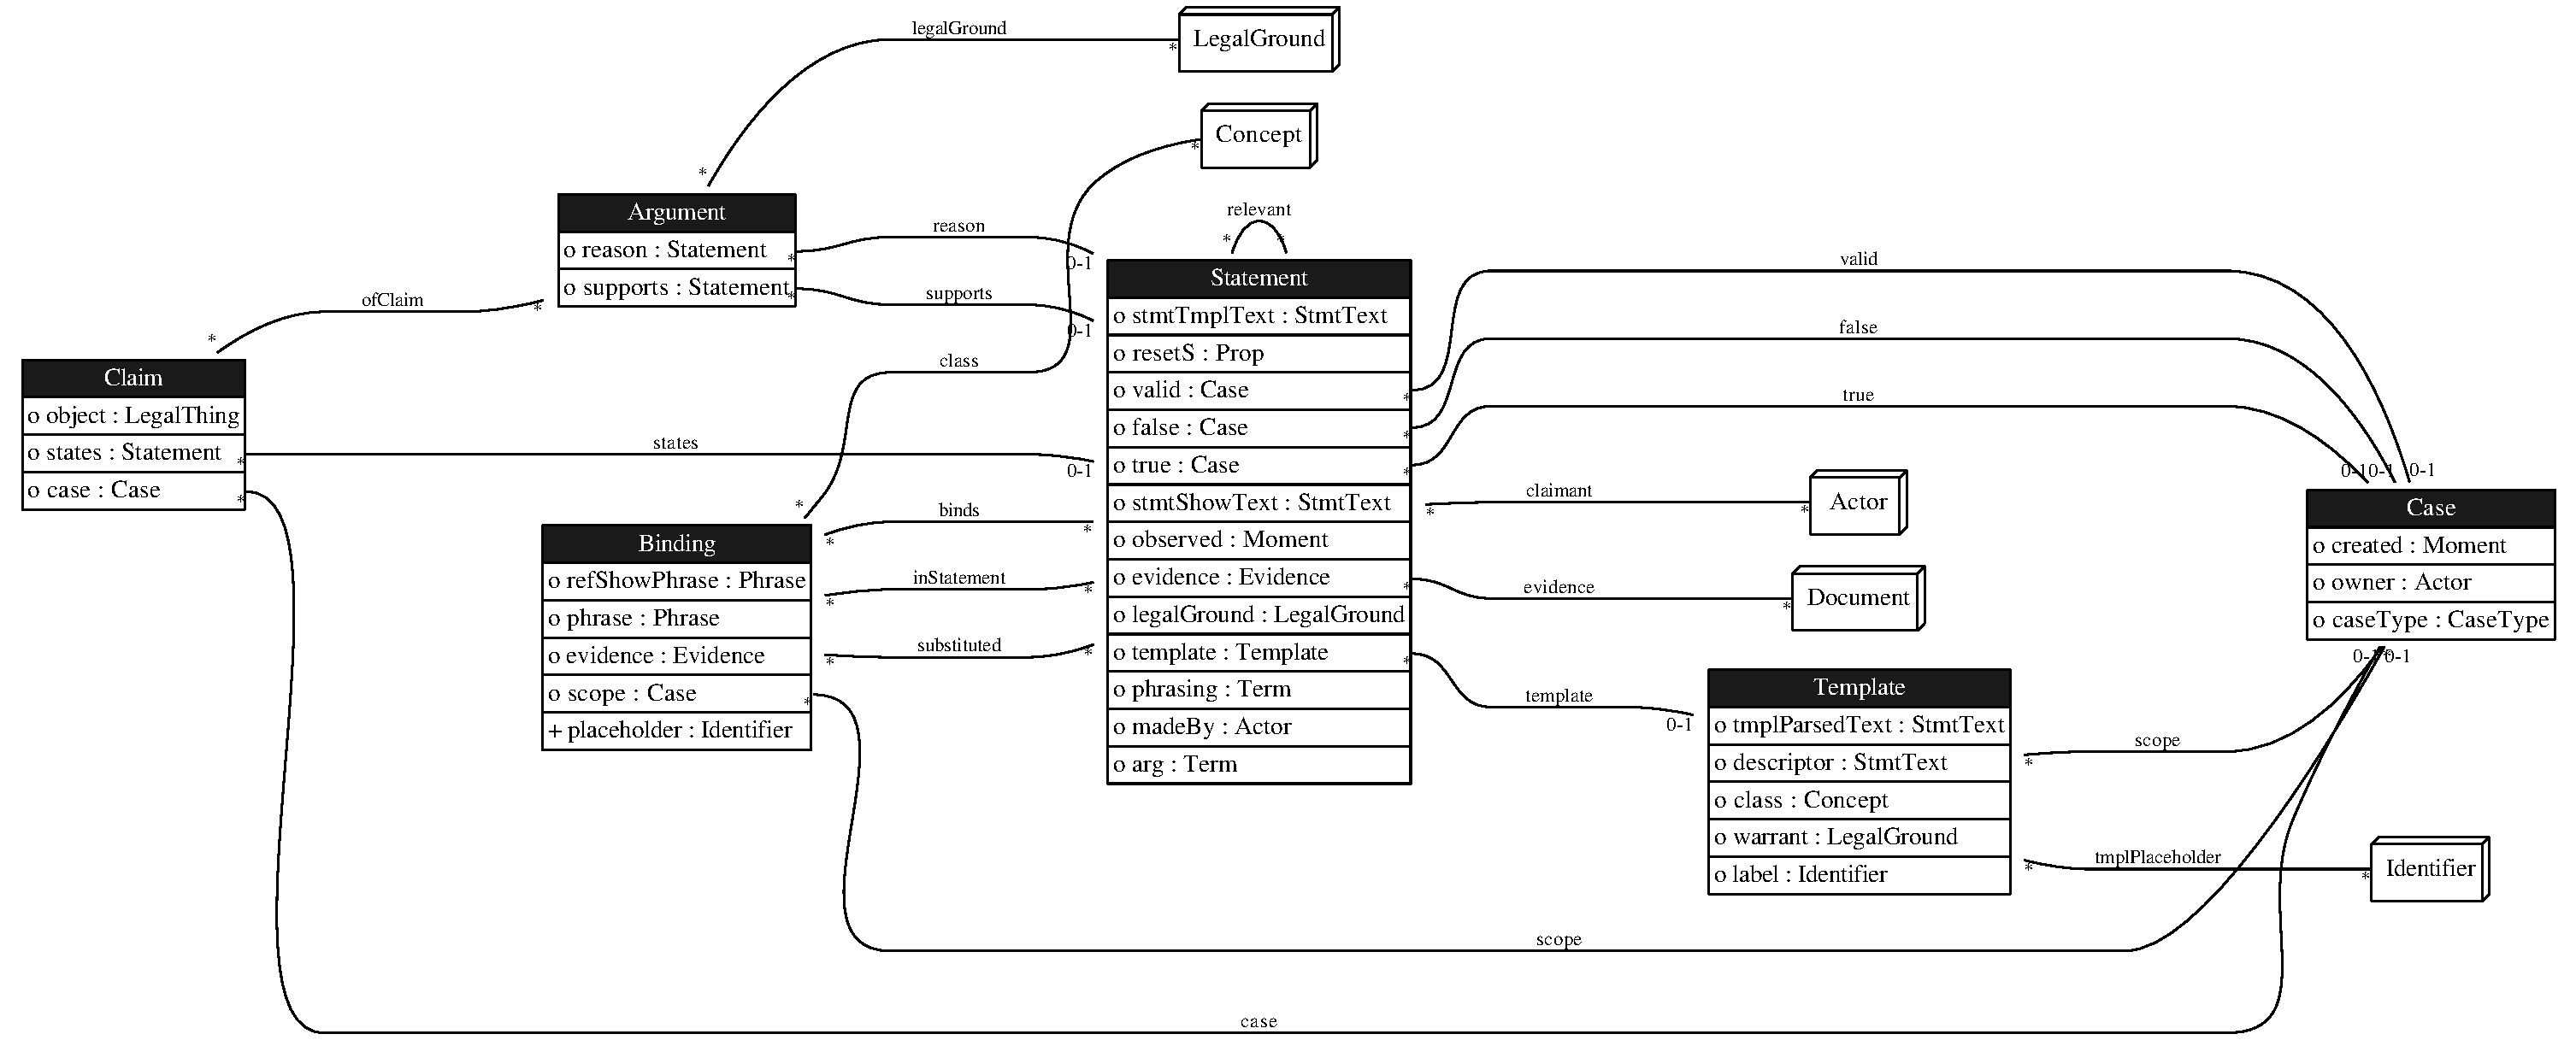
\includegraphics[scale=.23]{LogicalDataModel.pdf}
\end{center}
\caption{Conceptual data model}
\label{fig:conceptual model}
\end{figure}
	
	To convey the flavour of software development in relation algebra, it suffices to discuss a tiny part of the whole program.
	Therefore, we shall discuss the part of the conceptual model that is used in the sequel.
	The context in which a user creates arguments and reasons about them is a legal case.
	For this reason, validity, falsehood and truth of statements are related to the case.
	A \define{statement} is a phrase in natural language that can be either true or false.
	An example is \stmtText{The employee, John Brown, is entitled to 50 Euros}%
\footnote{This type of statement is typical for cases. It is valid only in the case where this particular John Brown is known.
	In other cases, where John Brown is unknown, this statement is meaningless}.
	In MirrorMe, a user can define a template, such as \stmtText{The employee, [emp], is entitled to [increase]}.
	The strings \stmtText{[emp]} and \stmtText{[increase]} are called placeholders.
	The reason for using placeholders is that legal rules are stated in general terms, e.g.
	\stmtText{Every employee is entitled to an increase in salary}.
	The user of MirrorMe will pick a legal text (from a source he trusts) and substitute parts of that text by placeholders.
	When the facts are known, the argument can be completed by substituting placeholders by actual phrases.

	It is precisely this substitution process that we have chosen to describe in this paper as a case study in
	programming with relation algebra.

\section{Programming in Relation Algebra}
\label{sct:Programming in RA}
	At this point we have reached the core of this case study.
	We focus on the substitution of placeholders when their values change.
	By focusing on this tiny detail, we can discuss the mechanics ``under the hood'' of the application generated by Ampersand.

	First we show how the computer solves the issue by looking at an exerpt of a log file (figure~\ref{fig:log file}).
	It shows an alternating sequence of the computer (ExecEngine) mentioning a rule,
	followed by insert or delete actions to satisfy that rule.
	Then we zoom in further, one rule at a time, to explain precisely what each rule looks like and how programming is done.
	We then discuss the same flow of events by means of a graph (figure~\ref{fig:event flow}) in which these rules and actions are nodes.
	This graph serves as an event flow diagram to illustrate the process behind figure~\ref{fig:log file}.

\begin{figure}[htb]
\begin{verbatim}
 ExecEngine run started
 ExecEngine satisfying rule 'signal phrase update'
 InsPair(resetS,Statement,Stat623,Statement,Stat623)
 ExecEngine satisfying rule 'flush substitutions'
 DelPair(substituted,Binding,Bind625,Statement,Stat623)
 ExecEngine satisfying rule 'reset statement text'
 InsPair(stmtShowText,Statement,Stat623,StmtText,
         The employee, [emp], is entitled to [increase].)
 ExecEngine satisfying rule 'done initializing'
 DelPair(resetS,Statement,Stat623,Statement,Stat623)
 ExecEngine satisfying rule 'substitute'
 InsPair(stmtShowText,Statement,Stat623,StmtText,
         The employee, James, is entitled to [increase].)
 InsPair(substituted,Binding,Bind625,Statement,Stat623)
 ExecEngine satisfying rule 'fill shownPhrase'
 InsPair(shownPhrase,Binding,Bind625,Phrase,James)
 ExecEngine run completed
\end{verbatim}
\caption{Log file of a substitution}
\label{fig:log file}
\end{figure}
	The log file of figure~\ref{fig:log file} has been taken from a computer that carries out the procedure to satisfy all rules.
	The machine will only act on rules that are violated.
	The first rule to be violated is ``signal phrase update'', in which the computer signals that something or someone has made a change
	in relation \id{phrase}.
	The procedure ends by doing the necessary substitutions,
	ensuring that all statements have the actual phrase of a placeholder in their text.

	Let us now study the actual rules to see how these rules cause the right actions to take place in the correct order.
	We will follow the log file from figure~\ref{fig:log file} in reverse direction,
	reasoning backwards from the result.

	Whether a placeholder has been edited can be observed by comparing its new phrase to the shown phrase%
\footnote{Note that we use the notion ``the phrase of a placeholder'' to indicate a pair from $\flip{\id{phrase}};\id{placeholder}$.}.
	The phrase of a placeholder is kept in the relation \id{phrase}.
	The shown phrase is kept in the relation \id{shownPhrase}.
	The sole purpose for having the relation \id{shownPhrase} is to detect a change in \id{phrase}.
	Let us introduce \id{differB} to represent the bindings with an updated phrase:
\[\id{differB} = \ident{Binding}\cap\id{shownPhrase};\cmpl{\ident{Phrase}};\flip{\id{phrase}}\]
	When the phrase of a placeholder changes,
	that phrase must be updated in every statement in which the placeholder was used.
	That update action is specified in section~\ref{rule: substitute}.
	Section~\ref{rule: fill shownPhrase} specifies how \id{shownPhrase} is made equal to \id{phrase},
	after all necessary substitutions are done.

\subsection{rule: fill shownPhrase}
\label{rule: fill shownPhrase}

\[\text{RULE}\ (\ident{Binding}\cap\id{substituted}/\id{inStatement} );\id{phrase}\ \subs\ \id{shownPhrase} \]
        This rule says that for each binding that has been substituted in every statement it is used in,
	the \id{phrase} must be equal to the \id{shownPhrase}.
	When violated, it is satisfied by inserting all violations into \id{shownPhrase}.

\subsection{rule: substitute}
\label{rule: substitute}
	Let us now look into the process of substituting placeholders by phrases.
	The relation \id{tmplParsedText} contains the original text, provided by a user.
	Placeholders are specified by enclosing them in brackets,
	e.g. \stmtText{The employee, [emp], is entitled to [increase]}.
	The text in which a placeholder has been substituted by a phrase,
	e.g. \stmtText{The employee, John Brown, is entitled to 50 Euros},
	is kept in relation \id{stmtShowText}.
	Each substitution that has been done in a statement corresponds to a binding-statement pair in the relation \id{substituted}.
	This relation keeps track of all substitutions.
	After a placeholder has been substituted, it no longer occurs in \id{stmtShowText}.
	This poses a problem if we want to substitute the new phrase in \id{stmtShowText}.
    For the placeholder that defines the place in the text where to substitute, is no longer in that text.
	Therefore, substitutions must be done in the original text of the statement.
	All placeholders in that text must then be substituted again.
	So, the text in \id{stmtShowText} must first be reset to the original text from \id{tmplParsedText}.
	To keep track of substitutions correctly, all corresponding binding-statement pairs must be removed from the relation \id{substituted}.
	Only after resetting is done, the substitutions can be put back in place with the new phrases filled in.
	
	We define a relation \id{resetS} to register the statements that are being reset.
    In statements that are not being reset, $\ident{Statement}-\id{resetS}$, substitutions can take place.
	All placeholders that have a binding with a phrase can be substituted. 
	The following rule specifies the action of substituting placeholders.
\begin{displaymath}
\begin{array}{rl}
\multicolumn{2}{l}{\text{RULE}}\\
&(\ident{Binding}\cap \id{phrase} ;\flip{\id{phrase}});\id{inStatement} ;(\ident{Statement} - \id{resetS})\\
\subs\\
&\id{substituted}
\end{array}
\end{displaymath}
	Violations of this rule are binding-statement pairs, of which the binding has a phrase and the statement is not being reset.
	Hence, this rule can be satisfied by inserting every violation into the relation substituted.

\subsection{rule: done initializing}
\label{rule: done initializing}
	Resetting a statement is done when two conditions are met.
	First, every statement that is (still) being reset may have no bindings in the relation \id{substituted}.
	Second, the text in \id{stmtShowText} corresponds to the text in \id{tmplParsedText}.
	So the rule that specifies the action is:

\begin{displaymath}
\begin{array}{rl}
\multicolumn{2}{l}{\text{RULE}}\\
&(\id{resetS} - \flip{\id{inStatement}};\id{substituted})\ \cap\\
&\id{template} ;\id{tmplParsedText} ;\flip{\id{stmtShowText}}\\
\subs\\
&\overline{\id{resetS}}
\end{array}
\end{displaymath}
	Violations of this rule are statements that are no longer being reset, but are still in the relation \id{resetS}.
	The appropriate action is to remove them from \id{resetS}.

\subsection{rule: reset statement text}
\label{rule: reset statement text}
	To satisfy one condition from section~\ref{rule: done initializing},
	the text in \id{stmtShowText} must be made equal to the original text in the template.
	The action is specified by the following rule:
\[\text{RULE}\ \id{resetS} ;\id{template} ;\id{descriptor}\ \subs\ \id{stmtShowText} \]
	Violations of this rule are descriptors of templates that belong to statements that are being reset.
	These violations can be resolved by inserting them in \id{stmtShowText}.

\subsection{rule: flush substitutions}
\label{rule: flush substitutions}
	To satisfy the other condition from section~\ref{rule: done initializing},
	the following rule specifies the action to be taken:
\[\text{RULE}\ \fullt{Binding}{Binding};\id{inStatement} ;\id{resetS}\ \subs\ \overline{\id{substituted} }\]
	Every binding in a statement that is being reset needs to be removed from the relation \id{substituted}.
	The software developer can implement this by deleting all violations of this rule from the relation \id{substituted}.

\subsection{rule: signal phrase update}
\label{rule: signal phrase update}
	When the phrase in a binding is edited and the new phrase differs from the shown phrase,
	this signals that substitutions must be flushed (see~\ref{rule: flush substitutions}),
	that the statement text must be reset to the original text (see~\ref{rule: reset statement text}),
	that the reset-state must be revoked (see~\ref{rule: done initializing}),
	that substitution must take place (see~\ref{rule: substitute}),
	and finally that the phrase detection is switched off again (see~\ref{rule: fill shownPhrase}).
	The initial condition occurs if a binding has been used (substituted) in a statement,
	and the binding satisfies \id{differB}.
	The following rule specifies the action that resetting a statment can start:
\[\text{RULE}\ \ident{Statement}\cap \flip{\id{inStatement}};\id{{\it differB}};\id{substituted}\ \subs\ \id{resetS} \]
	Violations of this rule are statements of which a substitution must be re-done.
	The software developer can have these violations added to \id{resetS} to satisfy this rule.
	In doing so, the chain of events is triggered that ends when all rules are satisfied.

\section{Programming in the Small}
\label{sct:Programming}
	Let us take a closer look at the programming process.
	Working in relation algebra, a software developer must think about satisfying constraints.
	She considers how violations arise from changing content of relations.
	And she thinks about insert and delete actions to resolve these violations.
	In our case study, we have reasoned with the event types: Ins $\la\id{relation}\ra$ and Del $\la\id{relation}\ra$%
\footnote{Ins and Del are called each others duals.}.
\begin{table}[htb]
{\small\begin{tabular}{|l|p{3.3in}|}\hline
rule&event types\\ \hline
signal phrase update&\small Ins \id{inStatement}, Ins \id{differB}, Ins \id{substituted}, Del \id{resetS}\\
flush substitutions&\small Ins \id{inStatement}, Ins \id{resetS}, Del \id{substituted}\\
reset statement text&\small Ins \id{resetS}, Ins \id{template}, Ins \id{descriptor}, Del \id{stmtShowText}\\
done initializing&\small Ins \id{resetS}, Del \id{inStatement}, Del \id{substituted}, Ins \id{template}, Ins \id{tmplParsedText}, Ins \id{stmtShowText}\\
substitute&\small Ins \id{phrase}, Ins \id{inStatement}, Del \id{resetS}, Del \id{substituted}\\
fill shownPhrase&\small Ins \id{substituted}, Del \id{inStatement}, Del \id{shownPhrase}, Ins \id{phrase}\\ \hline
\end{tabular}}
\caption{By which type of events can rules be violated?}
\label{fig:violation of rules}
\end{table}
	Table~\ref{fig:violation of rules} shows which event types may violate which rules.
	Recall section~\ref{sct:Programming in RA}, where the process of substitution started by updating the value of a placeholder.
	This meant doing an insert after a delete on the relation \id{phrase}, causing the updated phrase to appear in \id{differB}.
	That was signaled by the rule ``signal phrase update''.
\begin{figure}[bht]
\begin{center}
  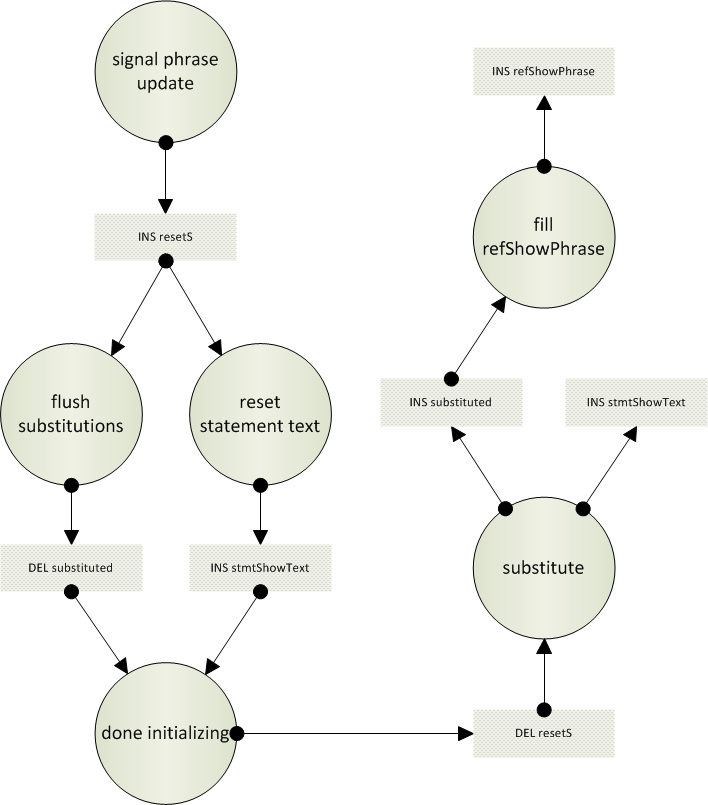
\includegraphics[scale=.55]{eventFlow.png}
\end{center}
\caption{event flow}
\label{fig:event flow}
\end{figure}
	In general, the software developer must decide how to resolve violations that occur as a result of some event.
	This can be done by choosing among the duals of the event types from table~\ref{fig:violation of rules}.
	By systematically swapping Ins for Del and vice-versa,
	the table shows by which type of events violations can be resolved.
	To ensure progress, the software developer will pick a different relation.
	For resolving the violations in the same relation would resolve the violations by undoing the change.
        Typically, preserving invariance of a rule is done by changing (one or more) different relations than the one that caused the violations.
	The software developer can draw a graph that contains all information from table~\ref{fig:violation of rules}
	and the dual information.
	Figure~\ref{fig:event flow} shows part of that graph.
	A circle represents a rule, a rectangle represents an event type, and the arrows connect them.
	The software developer can work her way through the graph, to write code to resolve violations for every event type that might occur.
	Figure~\ref{fig:event flow} shows just that part of the graph that corresponds with the case study in this article.

\section{Code Fragments}
\label{sct:Code Fragments}
	After the previous section, one question remains open: which code can preserve invariance and can we produce that code for arbitrary rules?
	We shall provide an answer to this question not just for the case study at hand, but for all conceivable cases.
	This section derives such code for every term in relation algebra.
	The problem of generating such code suffers from arbitrariness: there are many ways to generate correct code.
	We have not explored all possibilities, because there are too many.
	We do give one implementation for every conceivable term, pointing out where choices are to be made.

	The purpose of the code is to preserve invariance of rules by insertion and deletion into and from relations.
	Inserting (a set of) pairs $\Delta$ into a relation $r$ yields $r\cup\Delta$.
	Likewise, deleting pairs $\Delta$ from a relation $r$ yields $r-\Delta$.
	In this section we derive code for computers,
	which is built around two basic operations: insert and delete.
	The insert operation can be represented in terms of pre- and postconditions\footnote{this idea
	was introduced by Floyd and Hoare~\cite{Floyd1967,Hoare1969}.
	It is well known for making assertions about computer programs and reasoning about them.}.
\[\begin{array}{r@{~}l}
&\{\text{pre: }\code{P}=p\}\\
\code{INSERT}&\Delta\code{ IN P}\\
&\{\text{post: }\code{P}=p\cup\Delta\}\\
\end{array}\]

	The delete operation is introduced similarly:
\[\begin{array}{r@{~}l}
&\{\text{pre: }\code{P}=p\}\\
\code{DELETE}&\Delta\code{ FROM P}\\
&\{\text{post: }\code{P}=p-\Delta\}\\
\end{array}\]
	
	Let the following example introduce the idea of breaking and restoring invariance.
	Suppose the rule $\code{P}\subs\code{S}\cup\code{T}$ is to be kept satisfied by a computer,
	and \code{P}, \code{S}, and \code{T} are variables (memory locations) in that computer,
	which represent relations.
	We assume that before executing any code, we have $\code{P}=p$, $\code{S}=s$, and $\code{T}=t$.
	The following example shows that inserting a set of pairs, $\Delta$, in \code{P}
	may violate the rule.
	Inserting the same $\Delta$ in \code{S} restores invariance.
	In terms of code, we write:
\[\begin{array}{r@{~}l}
&\{\text{Assume $\code{P}=p$, $\code{S}=s$, $\code{T}=t$ and $\code{P}\subs\code{S}\cup\code{T}$}\}\\
\code{INSERT}&\Delta\code{ IN P}\\
&\{\text{$\code{P}=p\cup\Delta$, $\code{S}=s$, and $\code{T}=t$, and invariance is broken: $\code{P}\not\subs\code{S}\cup\code{T}$}\}\\
\code{INSERT}&\Delta\code{ IN S}\\
&\{\text{postcondition: $\code{P}=p\cup\Delta$, $\code{S}=s\cup\Delta$, $\code{T}=t$, and $\code{P}\subs\code{S}\cup\code{T}$}\}\\
\end{array}\]
	
	To prove that rule $\code{P}\subs\code{S}\cup\code{T}$ is kept satisfied,
	we must show that its value afterwards is equal to $\full$,
	under the condition that its initial value equals $\full$.
	The initial value is $\cmpl{p}\cup s\cup t$, which we may assume.
	The final value is $(p\cup\Delta)\subs(s\cup\Delta)\cup t$, which must be proven equal to $\full$:
\[\begin{array}{cl}
&(p\cup\Delta)\subs(s\cup\Delta)\cup t\\
=&\\
&\cmpl{p\cup\Delta}\ \cup\ s\ \cup\ \Delta\ \cup\ t\\
=&\hspace{1in}\{\hbox{De Morgan's law}\}\\
&(\cmpl{p}\cap\cmpl{\Delta})\ \cup\ s\ \cup\ \Delta\ \cup\ t\\
=&\hspace{1in}\{\hbox{Distribute $\cup$ over $\cap$}\}\\
&(\cmpl{p}\cup s\cup\Delta\cup t)\ \cap\ (\cmpl{\Delta}\cup s\cup\Delta\cup t)\\
=&\hspace{1in}\{\cmpl{\Delta}\cup\Delta=\full\}\\
&\cmpl{p}\cup s\cup\Delta\cup t\\
=&\hspace{1in}\{\full\ =\ \cmpl{p}\cup s\cup t\}\\
&\full
\end{array}\]
	From this derivation we may conclude that invariance of $\code{P}\subs\code{S}\cup\code{T}$ is restored.
	From this example, we can see that $\code{INSERT }\Delta\code{ IN T}$ would have worked just as well.
	In general, there are alternative ways of preserving invariance.
	This calls for a systematic analysis.
	The following sections analyze the various terms in Relation Algebra and provides some code to restore invariance of rules containing such terms.
	We start with an analysis of rules, then we proceed with boolean operators, and finally we arrive at relational operators.

\subsection{Implication Rules}
\label{ssct:Implication Rules}
	We will start by studying insertions and deletions in the simplest of rules:
\begin{equation}
\code{RULE }r\subs s\label{rule:r subs s}
\end{equation}
	Suppose an event occurs, e.g. $\Delta_r$ is inserted in $r$,
	and a programmer must write code that preserves invariance of rule~\ref{rule:r subs s}.
	This requires choosing a value for $\Delta_s$, such that equation~\ref{eqn:r subsRS s} holds:
\begin{eqnarray}
r\subs s&\Rightarrow&r\cup\Delta_r\subs s\cup \Delta_s\label{eqn:r subsRS s}
\end{eqnarray}
	The programmer can choose $\Delta_s=\Delta_r$, and call it just $\Delta$,
	satisfying equation~\ref{eqn:r subs s} trivially by monotonicity of $\subs$:
\begin{eqnarray}
r\subs s&\Rightarrow&r\cup\Delta\subs s\cup \Delta\label{eqn:r subs s}
\end{eqnarray}
	A programmer can take the antecedent of equation~\ref{eqn:r subs s}, $r\subs s$, as precondition.
	The consequent, $r\cup\Delta\subs s\cup \Delta$, is the postcondition.
	She then writes the following code fragment:
\[\begin{array}{r@{~}l}
&\{\text{Assume $\code{R}=r$, $\code{S}=s$, and $\code{R}\subs\code{S}$}\}\\
\code{INSERT}&\Delta\code{ INTO R};\\
&\{\text{$\code{R}=r\cup\Delta$, $\code{S}=s$, and $\code{R}\subs\code{S}$ is not necessarily true.}\}\\
\code{INSERT}&\Delta\code{ INTO S}\\
&\{\text{postcondition: $\code{R}=r\cup\Delta$, $\code{S}=s\cup\Delta$, and $\code{R}\subs\code{S}$}\}
\end{array}\]
	The first step, $\code{INSERT }\Delta\code{ INTO R}$, represents the event that may violate invariance of $\code{R}\subs\code{S}$.
	The second step, $\code{INSERT }\Delta\code{ INTO S}$, represents the reaction.

	A similar line of reasoning can be used for deletion as well:
\[\begin{array}{r@{~}l}
&\{\text{Assume $\code{R}=r$, $\code{S}=s$, and $\code{R}\subs\code{S}$}\}\\
\code{DELETE}&\Delta\code{ FROM S};\\
&\{\text{$\code{R}=r$, $\code{S}=s-\Delta$, and $\code{R}\subs\code{S}$ is not necessarily true.}\}\\
\code{DELETE}&\Delta\code{ FROM R}\\
&\{\text{postcondition: $\code{R}=r-\Delta$, $\code{S}=s-\Delta$, and $\code{R}\subs\code{S}$}\}
\end{array}\]
	The proof is noteworthy similar and equally trivial:
\begin{eqnarray}
r\subs s&\Rightarrow&r-\Delta\subs s-\Delta\label{eqn:r subs s by deletion}
\end{eqnarray}
	If the event is a deletion of $\Delta$ from $r$ or an insertion into $s$, no reaction is required.
	Such events cannot violate the invariance of rule~\ref{rule:r subs s},
	because equations~\ref{eqn:r subs s delfrom r} and~\ref{eqn:r subs s insinto s} hold for any $\Delta$:
\begin{eqnarray}
r\subs s&\Rightarrow&r-\Delta\subs s\label{eqn:r subs s delfrom r}\\
r\subs s&\Rightarrow&r\subs s\cup\Delta\label{eqn:r subs s insinto s}
\end{eqnarray}

Summarizing, some code for preserving invariance of rules of form $\code{R}\subs\code{S}$ is:
\[\begin{array}{|l|l|l|l|}
\hline
\text{invariant}&\text{action}&\text{reaction}&\text{eqn.}\\ \hline
\full=\code{R}\subs\code{S}&\code{INSERT}\ \Delta\code{ INTO R}&\code{INSERT }\Delta\code{ INTO S}&\ref{eqn:r subs s}\\
\full=\code{R}\subs\code{S}&\code{DELETE}\ \Delta\code{ FROM S}&\code{DELETE }\Delta\code{ FROM R}&\ref{eqn:r subs s by deletion}\\
\full=\code{R}\subs\code{S}&\code{DELETE}\ \Delta\code{ FROM R}&\code{Nop}&\ref{eqn:r subs s delfrom r}\\
\full=\code{R}\subs\code{S}&\code{INSERT}\ \Delta\code{ INTO S}&\code{Nop}&\ref{eqn:r subs s insinto s}\\ \hline
\end{array}\]
Preserving an invariant of the form $\code{R}=\code{S}$ is equivalent to preserving both $\code{R}\subs\code{S}$ and $\code{S}\subs\code{R}$ simultaneously.

\subsection{Rules with Boolean Operators}
	To write code for boolean expressions,
	we revert to the following lemma's:
\begin{eqnarray}
r=\cmpl{s}&\Rightarrow&r\cup\Delta=\cmpl{s-\Delta}\label{lbl:Preserve r = -s with Ins Delta into r}\\
r=\cmpl{s}&\Rightarrow&r-\Delta=\cmpl{s\cup\Delta}\label{lbl:Preserve r = -s with Del Delta from r}\\
t=r\cap s&\Rightarrow&t\cup\Delta=(r\cup\Delta)\cap(s\cup\Delta)\label{lbl:Preserve t=r inter s with Ins Delta into t}\\
t=r\cup s&\Rightarrow&t-\Delta=(r-\Delta)\cup(s-\Delta)\label{lbl:Preserve t=r union s with Del Delta from t}\\
t=r\cap s&\Rightarrow&t-\Delta=(r-\Delta)\cap s\label{lbl:Preserve t=r inter s with Del Delta from t}\\
t=r\cup s&\Rightarrow&t\cup\Delta=(r\cup\Delta)\cup s\label{lbl:Preserve t=r union s with Ins Delta into t}
\end{eqnarray}
	In proof assistant Isabelle, the proof of each of these lemmas is made in zero steps, so we omit these proofs here.

	Equations~\ref{lbl:Preserve r = -s with Ins Delta into r} and~\ref{lbl:Preserve r = -s with Del Delta from r}
	show that insertion in a term means deletion from its complement and vice versa.
	So the programmer can write the following code:
\[\begin{array}{r@{~}l}
&\{\text{Assume $\code{R}=r$, $\code{S}=s$, and $\code{R}=\cmpl{\code{S}}$}\}\\
\code{INSERT}&\Delta\code{ INTO R};\\
&\{\text{$\code{R}=r\cup\Delta$, $\code{S}=s$, and $\code{R}=\cmpl{\code{S}}$ is not necessarily true.}\}\\
\code{DELETE}&\Delta\code{ FROM S}\\
&\{\text{$\code{R}=r\cup\Delta$ and $\code{S}=s-\Delta$, so by eqn.~\ref{lbl:Preserve r = -s with Ins Delta into r} we have $\code{R}=\cmpl{\code{S}}$}\}
\end{array}\]
	Likewise, the reaction on a deletion will be an insertion:
\[\begin{array}{r@{~}l}
&\{\text{Assume $\code{R}=r$, $\code{S}=s$, and $\code{R}=\cmpl{\code{S}}$}\}\\
\code{DELETE}&\Delta\code{ FROM R};\\
&\{\text{$\code{R}=r-\Delta$, $\code{S}=s$, and $\code{R}=\cmpl{\code{S}}$ is not necessarily true.}\}\\
\code{INSERT}&\Delta\code{ INTO S}\\
&\{\code{R}=r-\Delta\text{ and }\code{S}=s\cup\Delta\text{, so by eqn.~\ref{lbl:Preserve r = -s with Del Delta from r} we have }\code{R}=\cmpl{\code{S}}\}
\end{array}\]

	Now consider equations~\ref{lbl:Preserve t=r inter s with Ins Delta into t} and~\ref{lbl:Preserve t=r union s with Del Delta from t}.
	If \code{T} changes, both \code{R} and \code{S} must be changed accordingly.
	Since $\cup$ and $\cap$ are associative operators, the arguments can be evaluated with no interaction between them.
	This allows us to define a primitive, \code{ALL}, without specifying in which order it processes its arguments\footnote{... leaving room to take advantage of parallelism.}.
	We define \code{ALL} to perform all actions from a given list:
\[\begin{array}{r@{~}l}
&\{\text{Assume }\forall\code{A}\in\code{AS}: (\{\id{pre}_{\code{\tiny A}}\}\ \code{A}\ \{\id{post}_{\code{\tiny A}}\})\text{ and } \id{pre}_{\code{\tiny A}} \}\\
\code{ALL}&\ \code{AS}\\
&\{\forall\code{A}: \id{post}_{\code{\tiny A}}\}
\end{array}\]
	With this primitive, we can write code for inserting pairs in \code{T},
	using equation~\ref{lbl:Preserve t=r inter s with Ins Delta into t}:
\[\begin{array}{r@{~}l}
&\{\text{Assume $\code{T}=t$, $\code{R}=r$, $\code{S}=s$, and $\code{T}=\code{R}\cap\code{S}$}\}\\
\code{INSERT}&\Delta\code{ INTO T};\\
&\{\text{$\code{T}=t\cup\Delta$, $\code{R}=r$, $\code{S}=s$ are true, but not necessarily $\code{T}=\code{R}\cap\code{S}$}\}\\
\code{ALL}&[\code{INSERT}\ \Delta\code{ INTO R},\code{INSERT}\ \Delta\code{ INTO S}]\\
&\{\code{R}=r\cup\Delta\text{ and }\code{S}=s\cup\Delta\text{, so by eqn.~\ref{lbl:Preserve t=r inter s with Ins Delta into t} we have }\code{T}=\code{R}\cap\code{S}\}
\end{array}\]
	Similarly, we can derive code for equation~\ref{lbl:Preserve t=r union s with Del Delta from t}:
\[\begin{array}{r@{~}l}
&\{\text{Assume $\code{T}=t$, $\code{R}=r$, $\code{S}=s$, and $\code{T}=\code{R}\cup\code{S}$}\}\\
\code{DELETE}&\Delta\code{ FROM T};\\
&\{\text{$\code{T}=t-\Delta$, $\code{R}=r$, $\code{S}=s$ are true, but not necessarily $\code{T}=\code{R}\cup\code{S}$}\}\\
\code{ALL}&[\code{DELETE}\ \Delta\code{ FROM R},\code{DELETE}\ \Delta\code{ FROM S}]\\
&\{\code{R}=r-\Delta\text{ and }\code{S}=s-\Delta\text{, so by eqn.~\ref{lbl:Preserve t=r union s with Del Delta from t} we have }\code{T}=\code{R}\cup\code{S}\}
\end{array}\]

	In equations~\ref{lbl:Preserve t=r inter s with Del Delta from t} and~\ref{lbl:Preserve t=r union s with Ins Delta into t},
	a choice must be made between $r$ and $s$. For that purpose we need a primitive \code{CHC} that chooses one action from a list $\code{AS}$, say $\code{A}$:
\[\begin{array}{r@{~}l}
&\{ (\{\id{pre}_{\code{\tiny A}}\}\ \code{A}\ \{\id{post}_{\code{\tiny A}}\})\text{ and } \id{pre}_{\code{\tiny A}} \}\\
\code{CHC}&\ \code{AS}\\
&\{\id{post}_{\code{\tiny A}}\}
\end{array}\]
	Note that this definition leaves open which term is selected.
	The following code shows how this works out for equation~\ref{lbl:Preserve t=r inter s with Del Delta from t}:
\[\begin{array}{r@{~}l}
&\{\text{Assume $\code{T}=t$, $\code{R}=r$, $\code{S}=s$, and $\code{T}=\code{R}\cap\code{S}$}\}\\
\code{DELETE}&\Delta\code{ FROM T};\\
&\{\text{$\code{T}=t-\Delta$, $\code{R}=r$, $\code{S}=s$ are true, but not necessarily $\code{T}=\code{R}\cap\code{S}$}\}\\
\code{CHC}&[\code{DELETE}\ \Delta\code{ FROM R},\code{DELETE}\ \Delta\code{ FROM S}]\\
&\{\text{Either }\code{R}=r-\Delta\text{ or }\code{S}=s-\Delta\text{, so by eqn.~\ref{lbl:Preserve t=r inter s with Del Delta from t} we have }\code{T}=\code{R}\cap\code{S}\}
\end{array}\]

	The following code shows how this works out for equation~\ref{lbl:Preserve t=r union s with Ins Delta into t}:
\[\begin{array}{r@{~}l}
&\{\text{Assume $\code{T}=t$, $\code{R}=r$, $\code{S}=s$, and $\code{T}=\code{R}\cup\code{S}$}\}\\
\code{INSERT}&\Delta\code{ INTO T};\\
&\{\text{$\code{T}=t\cup\Delta$, $\code{R}=r$, $\code{S}=s$ are true, but not necessarily $\code{T}=\code{R}\cup\code{S}$}\}\\
\code{CHC}&[\code{INSERT}\ \Delta\code{ INTO R},\code{INSERT}\ \Delta\code{ INTO S}]\\
&\{\text{Either }\code{R}=r\cup\Delta\text{ or }\code{S}=s\cup\Delta\text{, so by eqn.~\ref{lbl:Preserve t=r union s with Ins Delta into t} we have }\code{T}=\code{R}\cup\code{S}\}
\end{array}\]

	Section~\ref{ssct:Implication Rules} treated rules of the form $\code{R}\subs\code{S}$.
	Note that this rule can be rewritten to $\cmpl{\code{R}}\cup\code{S}=\full$.
	Consequently, rules did not have to be treated separately.
	We could have treated them as a special case of equations with boolean operators only.
	In fact, every rule with boolean operators $\cup$, $\cap$, and $-$ can be rewritten as a number of rules in disjunctive normal form\footnote{%
	Normalizing a boolean algebra is existing knowledge, and is considered outside the scope of this paper.} (DNF~\cite{davey1990}).
	We can represent a rule in DNF informally by:
\begin{eqnarray}
\code{RULE }\cmpl{r_0}\cup\ldots\cup\cmpl{r_n}\cup s_0\cup\ldots\cup s_m
\end{eqnarray}
	or more formally by
\begin{eqnarray}
\full=\cmpl{\bigcap\id{antecedents}}\cup\bigcup\id{consequents}
\end{eqnarray}
	in which \id{antecedents} are the complemented (negative) terms and \id{consequents} are the non-complemented (positive) terms.

	Summarizing, we have obtained code to preserve invariants in a boolean algebra:
\[\begin{array}{|l|l|l|l|}
\hline
\text{invariant}&\text{action}&\text{reaction}&\text{eqn.}\\ \hline
\code{R}=\cmpl{\code{S}}&\code{INSERT}\ \Delta\code{ INTO R}&\code{DELETE }\Delta\code{ FROM S}&\ref{lbl:Preserve r = -s with Ins Delta into r}\\
\code{R}=\cmpl{\code{S}}&\code{DELETE}\ \Delta\code{ FROM R}&\code{INSERT }\Delta\code{ INTO S}&\ref{lbl:Preserve r = -s with Del Delta from r}\\
\code{T}=\bigcap\code{TERMS}&\code{INSERT}\ \Delta\code{ INTO T}&\code{ALL }[\code{INSERT}\ \Delta\code{ INTO X}|\code{X}\in\code{TERMS}]&\ref{lbl:Preserve t=r inter s with Ins Delta into t}\\
\code{T}=\bigcup\code{TERMS}&\code{DELETE}\ \Delta\code{ FROM T}&\code{ALL }[\code{DELETE}\ \Delta\code{ FROM X}|\code{X}\in\code{TERMS}]&\ref{lbl:Preserve t=r union s with Del Delta from t}\\
\code{T}=\bigcap\code{TERMS}&\code{DELETE}\ \Delta\code{ FROM T}&\code{CHC }[\code{DELETE}\ \Delta\code{ FROM X}|\code{X}\in\code{TERMS}]&\ref{lbl:Preserve t=r inter s with Del Delta from t}\\
\code{T}=\bigcup\code{TERMS}&\code{INSERT}\ \Delta\code{ INTO T}&\code{CHC }[\code{INSERT}\ \Delta\code{ INTO X}|\code{X}\in\code{TERMS}]&\ref{lbl:Preserve t=r union s with Ins Delta into t}\\ \hline
\end{array}\]
	Having treated the boolean operators, let us consider code that is needed when relational operators are involved.

\subsection{Rules with relational operators}
	This section studies how to insert pairs into a term $r;s$.
	To formulate this precisely, we introduce an auxiliary relation $t$ to represent the term $r;s$.
	First we will insert pairs in $t$ while preserving invariance of $t=r;s$
	Then we will insert pairs in $r$ preserving the same rule.

	To insert pairs $\Delta$ into $t$ involves finding relations $\Delta_r$ and $\Delta_s$
	that satisfy equation~\ref{eqn:t subs r;s}.
\begin{equation}
t=r;s\ \Rightarrow\ t\cup\Delta=(r\cup \Delta_r);(s\cup \Delta_s)\label{eqn:t subs r;s}
\end{equation}
	Let us define a software primitive to compute both $\Delta_r$ and $\Delta_s$ and call it \code{NEWPAIRS}.
	It computes $\Delta_r$ and $\Delta_s$ from $r$, $s$, and $\Delta$.
	We can derive its postconditions from equation~\ref{eqn:t subs r;s} by means of the following derivation:
\[\begin{array}{r@{~}l}
&t\cup\Delta\\
=&\hspace{1in}\{\text{since }t\cup\Delta=t\cup(\Delta-t)\}\\
&t\cup(\Delta-t)\\
=&\hspace{1in}\{t=r;s\text{ and let \code{NEWPAIRS} ensure that }\Delta_r;\Delta_s=\Delta-t\}\\
&r;s\cup\Delta_r;\Delta_s\\
=&\hspace{1in}\{\text{let \code{NEWPAIRS} ensure that }r;\Delta_s\subs t\cup\Delta\text{ and }\Delta_r;s\subs t\cup\Delta\}\\
&r;s\cup r;\Delta_s\cup \Delta_r;s\cup \Delta_r;\Delta_s\\
=&\hspace{1in}\{\text{distributivity}\}\\
&(r\cup \Delta_r);(s\cup \Delta_s)
\end{array}\]
	The conditions in this derivation must be satisfied by \code{NEWPAIRS}. 
	This yields the following specification of \code{NEWPAIRS}:
\[\begin{array}{r@{~}l}
&\{\code{R}=r\text{ and }\code{S}=s\text{ and }\code{DELTA}=\Delta\}\\
\code{NEWPAIRS}&(\code{R}, \code{S}, \code{DELTA}): (\code{DELTAR}, \code{DELTAS})\\
&\{\code{DELTAR};\code{DELTAS}=\Delta\text{ and }\code{R};\code{DELTAS}\subs r;s\cup\Delta\text{ and }\code{DELTAR};\code{S}\subs r;s\cup\Delta\}
\end{array}\]
	The pre- and postconditions of \code{NEWPAIRS} are sufficient to satisfy equation~\ref{eqn:t subs r;s}.
	Since $t$ does not occur in the pre- and postconditions, \code{NEWPAIRS} implements equation~\ref{eqn:ins delta r;s}:
\begin{equation}
r;s\cup\Delta=(r\cup \Delta_r);(s\cup \Delta_s)\label{eqn:ins delta r;s}
\end{equation}
	Note that the specification of \code{NEWPAIRS} does not determine its implementation uniquely.
	There are multiple ways to implement \code{NEWPAIRS}.
	If \code{NEWPAIRS} creates one new pair for every pair in $\Delta-t$,
	we get $r;\Delta_s=\emptyset$ and $\Delta_r;s=\emptyset$.
	The weaker condition from the derivation, i.e. $r;\Delta_s\subs t\cup\Delta$ and $\Delta_r;s\subs t\cup\Delta$ allows some reuse of existing pairs.
	However, any implementation that preserves invariance of equation~\ref{eqn:ins delta r;s} will do.

	At this point we have the ingredients for code that preserves invariance of $\code{T}=\code{R};\code{S}$
\[\begin{array}{l}
\hspace{0.5in}\{\text{Assume }\code{R}=r\text{ and }\code{S}=s\text{ and }\code{T}=t\text{ and }\code{T}=\code{R};\code{S}\}\\
\code{INSERT }\Delta\code{ INTO T};\\
\hspace{0.5in}\{\code{R}=r\text{ and }\code{S}=s\text{ and }\code{T}=t\cup\Delta\text{, so }\code{T}\neq\code{R};\code{S}\}\\
(\code{DELTAR},\code{DELTAS})\code{ := }\code{NEWPAIRS}(\code{R}, \code{S}, \Delta-\code{T});\\
\hspace{0.5in}\{\code{R}=r\text{ and }\code{S}=s\text{ and }\code{T}=t\cup\Delta\text{ and }\\
\hspace{0.575in}\code{DELTAR};\code{DELTAS}=\Delta-\code{T}\text{ and }\\
\hspace{0.575in}\code{R};\code{DELTAS}\subs\code{T}\text{ and }\code{DELTAR};\code{S}\subs\code{T}\text{, so equation~\ref{eqn:ins delta r;s} is satisfied}\}\\
\code{INSERT DELTAR INTO R};\\
\hspace{0.5in}\{\code{R}=r\cup\code{DELTAR}\text{ and }\code{S}=s\text{ and }\code{T}=t\cup\Delta\}\\
\code{INSERT DELTAS INTO S}\\
\hspace{0.5in}\{\code{R}=r\cup\code{DELTAR}\text{ and }\code{S}=s\cup\code{DELTAS}\text{ and }\code{T}=t\cup\Delta\text{, so }\code{T}=\code{R};\code{S}\}
\end{array}\]
    This shows how to satisfy invariant $\code{T}=\code{R};\code{S}$ when pairs $\Delta$ are inserted into \code{T}.

	Let us now study how to keep $r;s$ constant when $r$ changes.
	Inserting pairs $\Delta$ into $r$ involves deleting pairs from $s$ such that:
\begin{equation}
(r\cup \Delta);(s-\Delta_s)=r;s\label{eqn:ins r del s}
\end{equation}
	In order to solve equation~\ref{eqn:ins r del s} towards $\Delta_s$,
	we derive\footnote{with thanks to Peter Jipsen, who pointed out this line of reasoning.}:
\begin{eqnarray}
&&(r\cup \Delta);(s-\Delta_s)\ \subs\ r;s\label{eqn:rs subs t by ins r del s}\\
&\Leftrightarrow&\nonumber\\
&&s-\Delta_s\ \subs\ (r\cup \Delta)\backslash(r;s)\nonumber\\
&\Leftrightarrow&\hspace{1in}\{\text{apply }x-y=z\ \Leftrightarrow\ x=z\cup y\text{ twice.}\}\nonumber\\
&&s-(r\cup \Delta)\backslash(r;s)\ \subs\ \Delta_s\nonumber
\end{eqnarray}
	This derivation shows that every solution $\Delta_s$ contains $s-(r\cup \Delta)\backslash(r;s)$.
	So the latter, $s-(r\cup \Delta)\backslash(r;s)$, is the smallest solution.

	The smallest solution might not contain all pairs from $r;s$.
	The missing pairs are $r;s-(r\cup\Delta);(s-(r\cup \Delta)\backslash(r;s))$.
	Therefore it may be necessary to reintroduce these missing pairs afterwards.
	Fortunately, we have just shown how to do just that with \code{NEWPAIRS}.
	This provides us with all the ingredients for code that preserves invariance of $\code{R};\code{S}=\code{T}$
\[\begin{array}{l}
\hspace{0.5in}\{\text{Assume }\code{R}=r\text{ and }\code{S}=s\text{ and }\code{T}=r;s\text{, so }\code{R};\code{S}=\code{T}\}\\
\code{INSERT }\Delta\code{ INTO R};\\
\hspace{0.5in}\{\code{R}=r\cup\Delta\text{ and }\code{S}=s\text{ and }\code{T}=r;s\text{, so }\code{R};\code{S}\neq\code{T}\}\\
\code{DELETE R}\backslash\code{T FROM S};\\
\hspace{0.5in}\{\text{Since }\code{R}=r\cup\Delta\text{ and }\code{T}=r;s\text{, we have }\code{R}\backslash\code{T}=(r\cup \Delta)\backslash(r;s)\\
\hspace{0.575in}\text{So }\code{S}=s-(r\cup \Delta)\backslash(r;s)\text{ and therefore}\\
\hspace{0.575in}\code{R};\code{S}\subs r;s\}\\
(\code{DELTAR},\code{DELTAS})\code{ := }\code{NEWPAIRS}(\code{R},\ \code{S},\ \code{T}-\code{R};\code{S});\\
\code{INSERT DELTAR INTO R};\\
\code{INSERT DELTAS INTO S}\\
\hspace{0.5in}\{\code{R};\code{S}=r;s\cup(\code{T}-\code{R};\code{S})=r;s\\
\hspace{0.575in}\text{so }\code{R};\code{S}=\code{T}\}
\end{array}\]

	Let us now study how to delete pairs $\Delta$ from $r$ while keeping $r;s$ constant.
	This involves inserting pairs into $s$ such that:
\begin{equation}
(r-\Delta);(s\cup\Delta_s)=r;s\label{eqn:del r ins s}
\end{equation}
	The largest solution of equation~\ref{eqn:del r ins s} follows from the law $x;(x\backslash y)\subs y$:
\begin{eqnarray}
&&x;(x\backslash y)\ \subs\ y\nonumber\\
&\Leftrightarrow&\hspace{1in}\{\text{Let }x=r-\Delta\text{ and }y=r;s)\}\nonumber\\
&&(r-\Delta);((r-\Delta)\backslash(r;s))\ \subs\ r;s\nonumber\\
&\Leftrightarrow&\hspace{1in}\{\text{Let }\Delta_s\ =\ (r-\Delta)\backslash(r;s)\}\nonumber\\
&&(r-\Delta);\Delta_s\ \subs\ r;s\nonumber\\
&\Leftrightarrow&\hspace{1in}\{p;x\subs p;q\ \Leftrightarrow\ p;(q\cup x)\subs p;q\}\nonumber\\
&&(r-\Delta);(s\cup\Delta_s)\ \subs\ r;s\nonumber
\end{eqnarray}
	This derivation shows that $(r-\Delta)\backslash(r;s)$, is the largest solution.

	Once again, we might not have all pairs from $r;s$,
	so eqn.~\ref{eqn:del r ins s} needs to be completed with the missing pairs.
	The missing pairs are $r;s-(r-\Delta);(s\cup(r-\Delta)\backslash(r;s))$.
	In this case too, these missing pairs can be reintroduced afterwards.
	This provides us with all the ingredients for code that preserves invariance of $\code{R};\code{S}=\code{T}$
\[\begin{array}{l}
\hspace{0.5in}\{\text{Assume }\code{R}=r\text{ and }\code{S}=s\text{ and }\code{T}=r;s\text{, so }\code{R};\code{S}=\code{T}\}\\
\code{DELETE }\Delta\code{ FROM R};\\
\hspace{0.5in}\{\code{R}=r-\Delta\text{ and }\code{S}=s\text{ and }\code{T}=r;s\text{, so possibly }\code{R};\code{S}\neq\code{T}\}\\
\code{INSERT R}\backslash\code{T INTO S};\\
\hspace{0.5in}\{\text{Since }\code{R}=r-\Delta\text{ and }\code{T}=r;s\text{, we have }\code{R}\backslash\code{T}=(r-\Delta)\backslash(r;s)\\
\hspace{0.575in}\text{So }\code{S}=s\cup(r-\Delta)\backslash(r;s)\text{ and therefore}\\
\hspace{0.575in}\code{R};\code{S}\subs r;s\}\\
(\code{DELTAR},\code{DELTAS})\code{ := }\code{NEWPAIRS}(\code{R},\ \code{S},\ \code{T}-\code{R};\code{S});\\
\code{INSERT DELTAR INTO R};\\
\code{INSERT DELTAS INTO S}\\
\hspace{0.5in}\{\code{R};\code{S}=r;s\cup(\code{T}-\code{R};\code{S})=r;s\\
\hspace{0.575in}\text{so }\code{R};\code{S}=\code{T}\}
\end{array}\]

	Summarizing, we have obtained some more code to preserve invariants in a relation algebra:
\[\begin{array}{|l|l|l|l|}
\hline
\text{invariants}&\text{action}&\text{reaction}&\text{eqn.}\\ \hline
\begin{array}{l}
\code{R};\code{S}\subs\code{T}\\
\code{S}\subs\code{R}\backslash\code{T}\\
\code{R}\subs\code{T}\slash\code{S}
\end{array}&\code{INSERT}\ \Delta\code{ INTO R}&\code{DELETE R}\backslash\code{T FROM S}&\ref{eqn:rs subs t by ins r del s}\\ \hline
\begin{array}{l}
\code{R};\code{S}\subs\code{T}\\
\code{S}\subs\code{R}\backslash\code{T}\\
\code{R}\subs\code{T}\slash\code{S}
\end{array}&\code{DELETE}\ \Delta\code{ FROM R}&\code{Nop}&\\ \hline
\code{T}\subs\code{R};\code{S}&\code{INSERT}\ \Delta\code{ INTO T}&
\begin{array}{l}
(\code{DELTAR},\code{DELTAS})\code{:=NEWPAIRS}(\code{R},\ \code{S},\ \Delta-\code{T});\\
\code{INSERT DELTAR INTO R};\\
\code{INSERT DELTAS INTO S}
\end{array}&\ref{eqn:ins delta r;s}\\ \hline
\code{T}\subs\code{R};\code{S}&\code{DELETE}\ \Delta\code{ FROM T}&\code{Nop}&\\ \hline
\code{T}\subs\code{R};\code{S}&\code{INSERT}\ \Delta\code{ INTO R}&\code{Nop}&\\ \hline
\code{T}\subs\code{R};\code{S}&\code{DELETE}\ \Delta\code{ FROM R}&\code{INSERT R}\backslash\code{T INTO S}&\\ \hline
\code{R};\code{S}=\code{T}&\code{INSERT}\ \Delta\code{ INTO R}&
\begin{array}{l}
\code{DELETE R}\backslash\code{T FROM S};\\
(\code{DELTAR},\code{DELTAS})\code{:=NEWPAIRS}(\code{R},\ \code{S},\ \code{T}-\code{R};\code{S});\\
\code{INSERT DELTAR INTO R};\\
\code{INSERT DELTAS INTO S}
\end{array}&\ref{eqn:ins r del s}\\ \hline
\code{R};\code{S}=\code{T}&\code{DELETE}\ \Delta\code{ FROM R}&
\begin{array}{l}
\code{INSERT R}\backslash\code{T INTO S};\\
(\code{DELTAR},\code{DELTAS})\code{:=NEWPAIRS}(\code{R},\ \code{S},\ \code{T}-\code{R};\code{S});\\
\code{INSERT DELTAR INTO R};\\
\code{INSERT DELTAS INTO S}
\end{array}&\ref{eqn:del r ins s}\\ \hline
\end{array}\]
	The solutions given here are far from being exhaustive.
	We illustrate this point by giving an example.
	Suppose we have $\code{T}\subs\code{R};\code{S}$ and action $\code{DELETE}\ \Delta\code{ FROM R}$.
	So the question is which pairs must be added to $s$ after pairs $\Delta$ have been removed from $r$.
	In normal circumstances, we might just look it up in the table above, picking $\code{INSERT R}\backslash\code{T INTO S}$ as a reaction.
	In the circumstance that initially $\code{T}=r;s$, we might reason differently.
	We must still find a smallest value for $\Delta_s$ that satisfies:
\begin{equation}
r;s\ \subs\ (r-\Delta);(s\cup\Delta_s)\label{lbl:nonshrinking r;s when Del from r}
\end{equation}
	The following derivation shows that $\flip{(r-\Delta)};(r\cap\Delta);s$ satisfies this requirement,
	but on one condition: for every pair in $r;s$ there must be a pair remaining behind in $r-\Delta$.
	Here is the derivation:
\begin{eqnarray}
&&\flip{(r-\Delta)};(r\cap\Delta);s\ \subs\ \Delta_s\nonumber\\
&\Rightarrow\nonumber\\
&&(r-\Delta);\flip{(r-\Delta)};(r\cap\Delta);s\ \subs\ (r-\Delta);\Delta_s\nonumber\\
&\Rightarrow&\hspace{1in}\{r;s;\flip{s};\flip{r} \cap\iden\ \ \subs\ (r-\Delta);\flip{(r-\Delta)}\}\nonumber\\
&&(r\cap\Delta);s\ \subs\ (r-\Delta);\Delta_s\nonumber\\
&\Leftrightarrow\nonumber\\
&&(r-(r-\Delta));s\ \subs\ (r-\Delta);\Delta_s\nonumber\\
&\Rightarrow\nonumber\\
&&(r;s)-((r-\Delta);s)\ \subs\ (r-\Delta);\Delta_s\nonumber\\
&\Leftrightarrow\nonumber\\
&&r;s\ \subs\ (r-\Delta);s \cup (r-\Delta);\Delta_s\nonumber\\
&\Leftrightarrow\nonumber\\
&&r;s\ \subs\ (r-\Delta);(s \cup \Delta_s)\nonumber
\end{eqnarray}
	This derivation justifies the reaction $\code{INSERT }\flip{(r-\Delta)};(r\cap\Delta);s\code{ INTO S}$,
	but only if $r;s;\flip{s};\flip{r} \cap\iden\ \ \subs\ (r-\Delta);\flip{(r-\Delta)}$.

\section{Reflection}
\label{sct:Reflection}
	Ampersand is being built on the belief that software development should be automated.
	The holy grail is to derive deterministic ways to preserve invariants, to allow for programming by constraints.
	This is motivated by the benefits of describing a result in terms of constraints,
	rather than having to invent all the steps that lead to that result.
	For example, describing the situation that any financial transaction must preserve the total amount of money is simpler
	than having to describe all the steps involved in such a transaction.
	The attraction is not only for the programmer, but even more so for auditors and users for who the constraints are easier to grasp and validate.
	In this paper we have shown how to derive specific steps,
	helping the programmer to invent code and providing mathematical assurance of correctness (compliance-by-design).

	The analysis in this paper shows once more that inventing algorithms for preserving invariants is far from trivial.
	Algorithms cannot be derived from constraints alone. The choices that remain must be resolved first.
	This paper does show, however, that these choices occur in predictable ways.
	That gives opportunities, for instance to make these choices explicit to a user, to optimize the number of choices,
	or to use external knowledge to resolve the remaining choices on runtime.

	In practice we have experienced that programming by constraints in relation algebra yields an unconventional way of programming.
	This experience consists of inventing rules and choosing event types for resolving violations, as illustrated by the case study.
	To relate this experience to programming as we know it, section~\ref{sct:Comparison} makes a comparison with established programming languages (prior art).
	Section~\ref{sct:Contribution} summarizes the contributions to software development claimed by Ampersand.
	Section~\ref{sct:Ampersand in practice} summarizes the use of Ampersand in practice and
	section~\ref{sct:Further Research} gives an outlook on research that is required in the near future.

\subsection{Comparison}
\label{sct:Comparison}
	This section compares Ampersand with existing programming paradigms by mentioning the most important differences and similarities.

	The first to compare with is the imperative programming paradigm, known from popular languages such as Java~\cite{Java} and C++~\cite{Stroustrup97a}.
	Our case study cannot be called imperative, because the notion of control flow in imperative languages is very different.
	In imperative languages, the control flow is defined by the software developer.
	In this case study, the control flow emerges as a result of changes in relation content as illustrated
	by figure~\ref{fig:event flow}.

	The case study also differs from the logic programming paradigm of Prolog~\cite{Lloyd1984} and of all rule engines that can be considered to be an offspring of Prolog.
	A difference lies in the way rules are interpreted.
	In logic programming, a program consists of Horn-clauses and a resolution-proof is constructed on run-time.
	The software developer works with notions such as backtracking (backward chaining) and unification, which are absent in Ampersand.
	Ampersand is not restricted to Horn-clauses; any relation-algebraic equation over relations can be used as a rule.

	The case study also differs from functional programming, of which Haskell and Scala are prominent representants.
	A core idea in functional programming is to evaluate a program as a function from input to output~\cite{Backus1978}.
	A functional program consists of function definitions, that are evaluated by a term- or graph-rewriter, using various strategies such as lazy or eager evaluation.
	In contrast, one might interpret our case study as a relaxation of the constraint that everything is a function.
	In relation algebra, everything is a relation and a function is a restricted form of a relation.
	A similarity to functional programming is the declarative style, because substitution of equal terms without changing the semantics is a property we see in both worlds.

	A difference with database programming is found in the type of algebra that is used.
	Relational databases are founded on relational algebra~\cite{Codd70}. They are typically programmed in SQL.
	In contrast with database programming, Ampersand implements heterogeneous relation algebra~\cite{Schmidt1997}.
	A software developer working with relational algebra sees n-ary tables, while Ampersand is restricted to binary relations.
	The comparison between relation{\it al} algebra and relation algebra might relate to comparing relational databases with graph databases~\cite{Vicknair2010},
	although no literature was found to corroborate this.

	In the tradition of formal specification, there are many relational approaches, such as Z~\cite{Z}, CSP~\cite{CSP}, LOTOS~\cite{LOTOS}, VDM~\cite{VDM}.
	Where formal specification techniques typically analyse and diagnose specifications,
	Ampersand actually synthesizes (generates) information systems.

	The similarity with the reactive programming paradigm~\cite{Bainomugisha2013} is obvious from figure~\ref{fig:event flow}.
	This graph is part of the program graph as conceived in reactive programs.
	The code fragments described in section~\ref{sct:Code Fragments}
	might be generated towards a mature reactive programming language (e.g. ELM)
	and executed directly.
	Ampersand lets you think in constraints and (reactive) code fragments to preserve invariants can be generated with the theory in this paper.
	Currently Ampersand generates towards classical PHP+HTML+JavaScript code,
	but generation to a reactive programming language (e.g. ELM) is definitely on the wishlist.

	If Ampersand represents a programming style at all, we might call it a relation-algebraic style of programming or maybe constraint programming\footnote{https://en.wikipedia.org/wiki/Constraint\_programming}.
	Ampersand's style would be characterized by a programmer who specifies constraints and a computer trying to satisfy these constraints by resolving violations.

\subsection{Contribution}
\label{sct:Contribution}
	Contributions of Ampersand to the software development process are:
\begin{itemize}
\item	Ampersand has the usual benefits of a declarative language:
	This means that terms can be manipulated by Tarski's axioms without changing their semantics~\cite{vdWoude2011}.
	It also means that the order in which rules are written has no consequence for their semantics.
\item	Heterogeneous relation algebra has a straightforward interpretation in natural language~\cite{RBD}.
	We have used that to formalize business requirements without exposing business stakeholders to any formal notation.
\item	Heterogeneous relation algebra in Ampersand is statically typed~\cite{Joosten2015}.
	There is much evidence for significantly lower software maintenance cost due to static typing as opposed to dynamic typing~\cite{HanenbergKRTS14,Petersen2014}.
\item	Heterogeneous relation algebra is well studied.
	As a consequence, many tools that are readily available in the public domain can be put to good use.
	For executives of large organizations it can be reassuring that the formalism is free of childhood diseases.
\item	Relation algebra facilitates composing software from reusable components, because a program consists of rules.
	Since the union of sets of rules is a set of rules, compositionality comes from the union operator.
	In practice, when components are brought together in larger assemblies, hardly any adjustments have to be made%
\footnote{This is (unsubstantiated) experience collected from projects we have done with Ampersand.}.
\end{itemize}

	Ampersand also has disadvantages. It appears to be difficult to learn for large groups of software professionals.
	Research~\cite{Michels2015} shows that this is largely due to deficits in prerequisite knowledge, especially skills in discrete mathematics.
%	For this reason, we have made an addendum to the course we teach at the Open University of the Netherlands.
	Also, programming appears to be difficult in practice.

\subsection{Ampersand in Practice}
\label{sct:Ampersand in practice}
	Ampersand has been used in practice both in education (Open University of the Netherlands)
	and in industry (Ordina and TNO).
	For example, Ordina designed a proof-of-concept in 2007 of the INDIGO-system,
	which is still in use today as the core information system of the Dutch immigration authority, IND.
	The design of INDIGO was made with Ampersand, to obtain correct, detailed results in the least amount of time.
	More recently, Ampersand was used to design an information system called DTV for the Dutch food authority, NVWA.
	A prototype of DTV was built by Ampersand and was used as a model to build the actual system.
	TNO, a major Dutch industrial research laboratory, is using Ampersand for research purposes.
	For example, TNO did a study of international standardizations efforts such as
	RBAC (Role Based Access Control) in 2003 and architecture (IEEE 1471-2000)~\cite{IEEE1471} in 2004.
	Several inconsistencies were found in the last (draft) RBAC standard~\cite{RBAC}.
	TNO has also used the technique in conceiving several patents%
\footnote{e.g. patents DE60218042D, WO2006126875, EP1727327, WO2004046848, EP1563361, NL1023394C, EP1420323, WO03007571, and NL1013450C.}.
	At the Open University of the Netherlands, Ampersand is being taught in a course called Rule Based Design~\cite{RBD}.
	In this course, students use a platform called RAP, which has been built in Ampersand~\cite{Michels2015}.
	RAP has been the first Ampersand-application that has run in production.

\subsection{Further Research}
\label{sct:Further Research}
	Further research on this topic is required to bring relation algebra still closer to the community of practitioners.
	Further use of relation algebra can be made by incorporating a model checker, such as the Alloy analyser~\cite{Alloy2006}, to detect inconsistent rules.
	An exciting new development is Amperspiegel~\cite{Amperspiegel}, which brings notational flexibility at the fingertips of the user.
	Developments in the Ampersand-compiler are going towards a rule-repository (written in Ampersand itself).
	This will make collaborative information systems development in Ampersand easier, because the repository can assist in automating
	the software development process further.
	Other research is needed towards a comprehensive theory of information systems.
	Currently, there is no theory (in the mathematical meaning of the word) for information systems.
	In the Ampersand project, a sub-project called ``Formal Ampersand'' is being conducted to achieve this goal.
\subsection{Acknowledgements}
\label{sct:Acknowledgements}
	Firstly, I wish to thank Sebastiaan Joosten for introducing me to Isabelle and for inspiring me with his challenging critiques.
	I owe many thanks to Wolfram Kahl, Michiel Stornebrink, Han Joosten, and the anonymous reviewers of RAMiCS for their useful feedback.
	And I am very grateful to the Open University and Ordina for funding this research.

\section{Bibliography}
\bibliographystyle{elsarticle-harv}
\bibliography{doc}


\end{document}
